\cleardoublepage

\chapter{ImageCLEF Lifelog Challenge}
\label{ch:imageclef}

This chapter aims at describing the ImageCLEF Lifelog challenge. Firstly in Section \ref{sec:introduct} an introduction is given to the challenge and the respective goals. Section \ref{sec:tasks} describes the tasks available for the year 2020. The concept of lifelogging is explained in Section \ref{sec:concept_lifelog}. Finally Section \ref{sec:imagecleflifelog} clarifies the Lifelog Moment Retrieval Task (LMRT) which is the main focus of this work, along with an introduction to the dataset, dev topics, test topics, ground truth and the evaluation methodology of the task.



\section{The ImageCLEF challenge}
\label{sec:introduct}

The ImageCLEF challenge is a large–scale evaluation campaign that aims at evaluating cross-language image retrieval systems. It is organized as part of the CLEF Initiative (Conference and Labs of the Evaluation Forum, formerly known as Cross-Language Evaluation Forum) and launched in  2003. Initially proposed by Mark Sanderson and Paul Clough from the Department of Information Studies from the University of Sheffiel with the goal of providing support for the evaluation of 1) language-independent methods for the automatic annotation of images with concepts, 2) multimodal information retrieval methods based on the combination of visual and textual features, and 3) multilingual image retrieval methods, so as to compare the effect of retrieval of image annotations and query formulations in several languages.


Every year an evaluation cycle campaign occurs that consist in workshops where teams can compete to achieve the best possible results while discussing new techniques and ideas. In addition to offering the evaluation platform, ImageCLEF also provides several publicly resources, such as benchmarks to evaluate retrieval systems. These benchmarks have helped researchers develop new approaches to visual information retrieval and automatic annotation by enabling the performance of various approaches to be assessed.

Since the launch of ImageCLEF, researchers within academic and commercial research groups worldwide, including those from Cross–Language Information Retrieval (CLIR), medical informatics, Content–Based Image Retrieval (CBIR), computer vision and user interaction have been participating in the challenge. 

Currently, ImageCLEF main goal is to support the advancement of the field of visual media analysis, indexing, classification, and retrieval, by developing the necessary infrastructure for the evaluation of visual information retrieval systems operating in both monolingual, cross–language and language-independent contexts \cite{Zhang2008}. 


\newpage
\section{The Tasks}
\label{sec:tasks}

The ImageCLEF 2020 edition presents 4 different tasks:
    \begin{itemize}
    \item \textbf{ImageCLEFlifelog}: Addresses the problems of lifelogging data retrieval and summarization. The work done in this thesis aims at participating in this task, therefore this task can be read in more detail in Section \ref{sec:imagecleflifelog}.
    
    \item \textbf{ImageCLEFcoral}: Addresses the problem of automatically segmenting and labeling a collection of images that can be used in combination to create 3D models for the monitoring of coral reefs.
    
    \item \textbf{ImageCLEFmedical}: The task combines the most popular medical tasks of ImageCLEF and continues the last year idea of combining various applications, namely: automatic image captioning and scene understanding, medical visual question answering and decision support on tuberculosis. This allows to explore synergies between the tasks.
    
    \item \textbf{ImageCLEFdrawnUI}: The task addresses the problem of automatically recognizing hand drawn objects representing website UIs, that will be further translated into automatic website code.
    \end{itemize}


\section{The concept of lifelogging}
\label{sec:concept_lifelog}

Lifelogging is defined as a form of pervasive computing consisting of a unified digital record of the totality of an individual’s experiences, captured multimodally through digital sensors and stored permanently as a personal multimedia archive. In a simple way, lifelogging is the process of tracking and recording personal data created through our activities and behaviour.

Personal lifelogs have a great potential in numerous applications, including memory and moments retrieval, daily living understanding, diet monitoring, or disease diagnosis, as well as other emerging application areas. For example: in Alzheimer’s disease, people with memory problems can use a lifelog application to help a specialist follow the progress of the disease, or to remember certain moments from the last days, weeks or even months.

One of the greatest challenges of lifelog applications is the large amount of lifelog data that a person can generate. The lifelog datasets, for example the ImageCLEFlifelog dataset, are rich multimodal datasets which consist in one or more months of data from multiple lifeloggers. Therefore, an important aspect is the lifelog data organization in the interest of improving the search and retrieval of information. In order to organize the lifelog data, useful information has to be extracted from it \cite{Ribeiro2019} \cite{Ribeiro2020}.

\newpage
\section{ImageCLEFlifelog}

\label{sec:imagecleflifelog}


The ImageCLEFlifelog 2020 task is divided into two different sub-tasks: the Lifelog moment retrieval (LMRT) and Sport Performance Lifelog (SPLL) sub-task. In this work, as in the previous year’s challenge, it was only addressed the LMRT sub-task, as a continuous research work that is intended to be developed with the aim of giving a contribution to real problems that exist around the world that can benefit from this technology.
    
The UA.PT Bioinformatics, a team from the Institute of Electronics Engineering and Telematics in the University of Aveiro, participated in the LMRT subtask with two different retrieval systems. The first one is the automatic retrieval system which was a continuation of the work done in the previous year challenge \cite{Ribeiro2019} and the main objective of this thesis. The other one was a retrieval system capable of providing user interaction and visualization. 

The interactive retrieval system is only interesting for this work in terms of comparing the achieved results, therefore this document will only give a small description of this system in Chapter \ref{ch:results} Section \ref{sec:overall_perfomance}. More details are presented in \cite{Ribeiro2020}.

    \subsection{SubTask: Lifelog Moment Retrieval}
    In the LMRT subtask, the main objective is to create a system capable of retrieving a number of predefined moments in a lifelogger’s day-to-day life from a set of images. Moments can be defined as semantic events or activities that happen at any given time during the day. For example, given the query “Find the moment(s) when the lifelogger was having an icecream on the beach” the participants should return the corresponding relevant images that show the moments of the lifelogger having icecream at the beach. Like last year, particular attention should be paid to the diversification of the selected moments with respect to the target scenario.

    ImageCLEFlifelog dataset is a rich multimodal dataset which consists of 4.5 months of data from three lifeloggers, namely: images (1,500-2,500 per day), visual concepts (automatically extracted visual concepts with varying rates of accuracy), semantic content (locations and activities) based on sensor readings on mobile devices (via the Moves App), biometrics information (heart rate, galvanic skin response, calories burn, steps, continual blood glucose, etc.), music listening history and computer usage. 
    Except for the images, all of the data was provided in a csv file. An excerpt of this file is presented in Figure \ref{fig:dataset_csv} and examples of images from the dataset are showcased in Figure \ref{fig:dataset_image}.

    \begin{figure}[htb]
        
        \centering
 
        \captionsetup{justification=centering}
        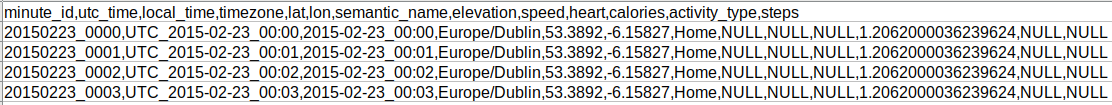
\includegraphics[width =  \textwidth]{Sections/5ImageClef/images/dataset.png}
        \caption[Provided csv file.]{Excerpt of the csv file provided by the organizers.}  
       \label{fig:dataset_csv}
    \end{figure}


    \begin{figure}[H]
        \captionsetup{justification=centering}
        \begin{subfigure}{\linewidth}
        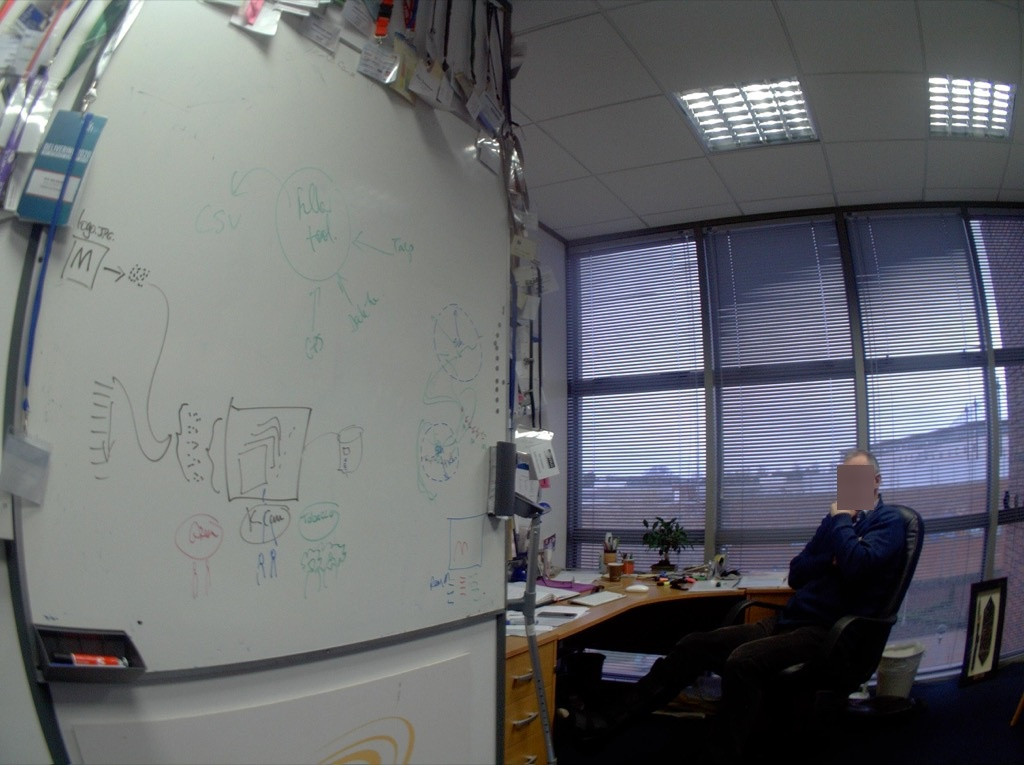
\includegraphics[width=.3\linewidth]{Sections/5ImageClef/images/image1.jpg}
        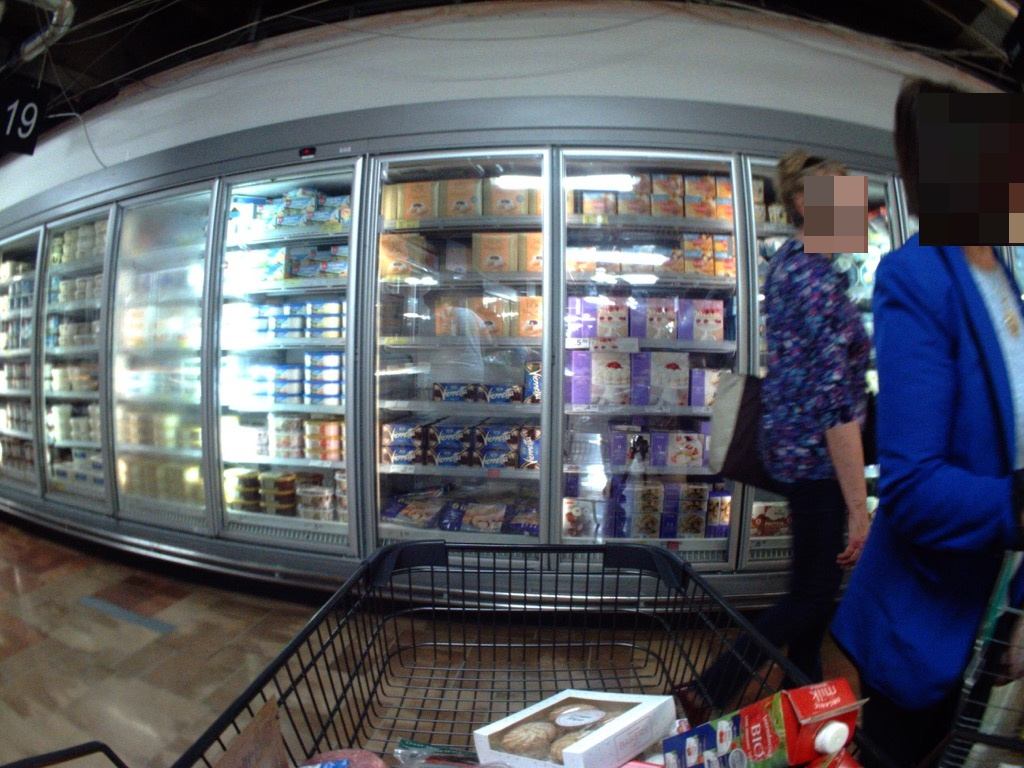
\includegraphics[width=.3\linewidth]{Sections/5ImageClef/images/image2.jpg}
        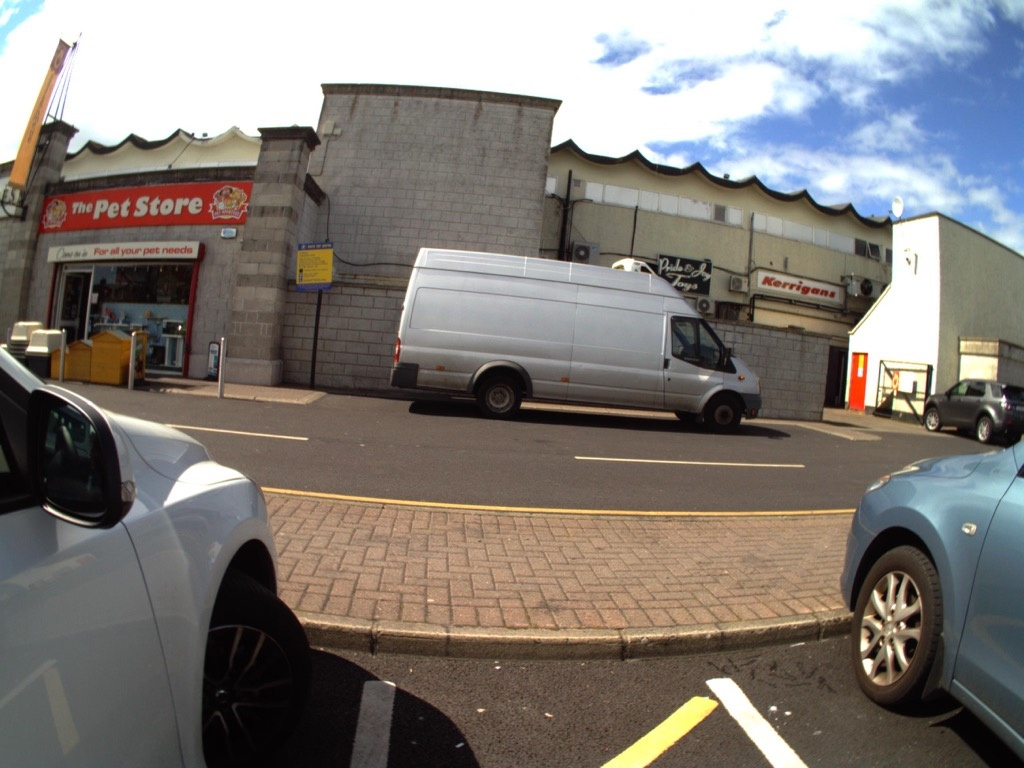
\includegraphics[width=.3\linewidth]{Sections/5ImageClef/images/image3.jpg}
        \end{subfigure}\par\medskip
        \begin{subfigure}{\linewidth}
        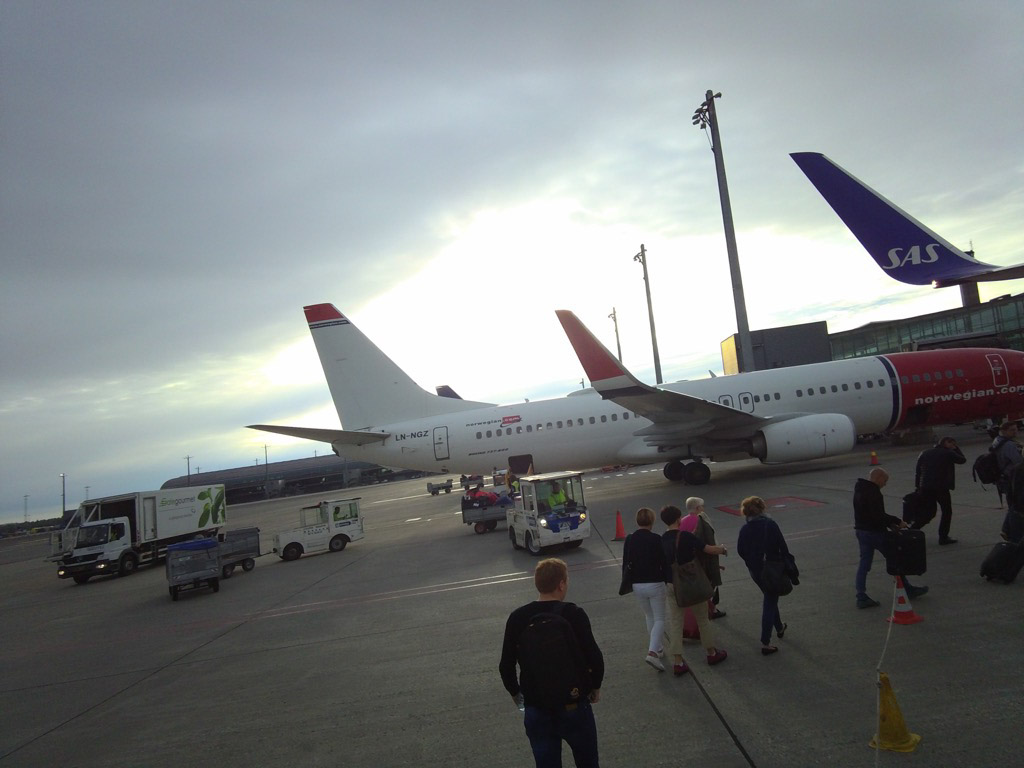
\includegraphics[width=.3\linewidth]{Sections/5ImageClef/images/image4.jpg}
        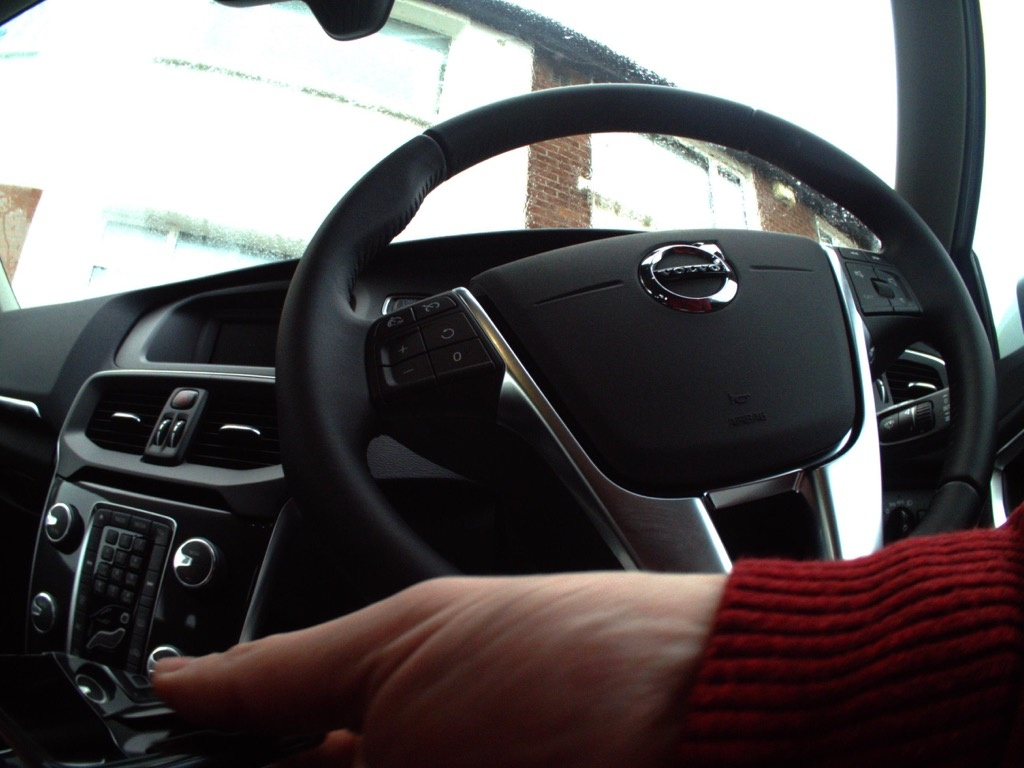
\includegraphics[width=.3\linewidth]{Sections/5ImageClef/images/image5.jpg}
        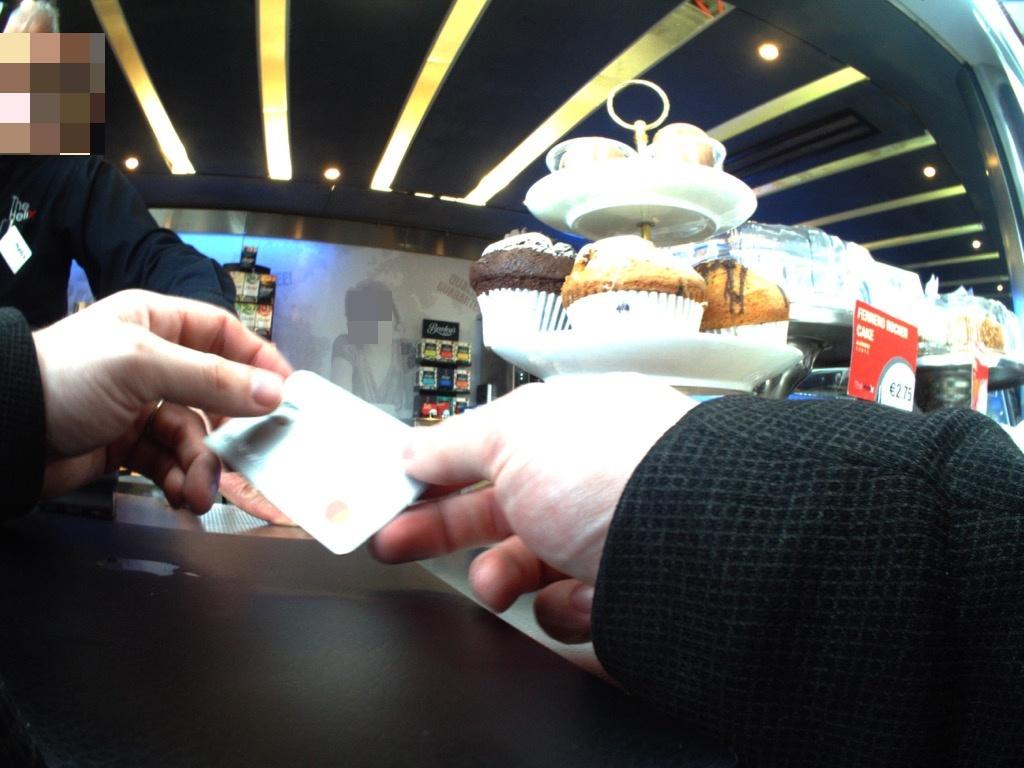
\includegraphics[width=.3\linewidth]{Sections/5ImageClef/images/image6.jpg}
        \end{subfigure}\par\medskip
        \caption[Images from the imageCLEF dataset]{Example of images from the imageCLEF dataset.}
        \label{fig:dataset_image}
      \end{figure}


    
    In this work only the images, the respective semantic content and time were used \cite{Ribeiro2020}. This decision is mainly justified by the fact that much of the provided data like the biometric information, computer usage and music history gives no useful information for the retrieval of images. The visual concepts provided were also not utilized since the system created in this work uses its own algorithms in order to extract more accurate labels from the images. 
    

    Initially, the dev topics are firstly released along with the images dataset and the corresponding ground truth. This means that it is possible to initially create a retrieval system and analyse if it is producing good results, since thanks to the ground truth it is known which pictures should be retrieved for each textual topic. 

    After a few weeks the test topics for evaluation are released without the ground truth, the participants who achieve the best results are the ones who have the highest F1-measure at the top 10 images score. This is further discussed in Section \ref{sec:eval}.
    \newpage
    \subsection{Dev Topic example}
    \label{sec:devtopic1}
    As discussed above the participants should return the corresponding relevant images that show the moments of the lifelogger during a predefined moment. 
    
    Those moments are provided in the format of a pdf file that contains 10 different textual query topics representing 10 different moments. Topic 1 is illustrated below to serve as an example of the query topics:
    


   \hfill

        \textbf{Title} : ``Having Beers in a Bar”

        \textbf{Description} : ``Find the moment in 2015 and 2016 when u1 enjoyed beers in the bar.”

        \textbf{Narrative} : ``To be considered relevant, u1 must be clearly in a bar. Any moments that u1 drinks beers at home or outside without the bar view are not considered relevant.”
        


    
    \begin{itemize}
        \item    \textbf{Example of the ground truth}
    \end{itemize}
 


    The ground truth is given as text file with the following format : \textbf{[topic number, image name, cluster]}.
    The cluster number is used to calculate the F1-measure score which will be explained in more detail in Section \ref{sec:eval}.


    \begin{figure}[htb]
        
        \centering
        \captionsetup{justification=centering}
        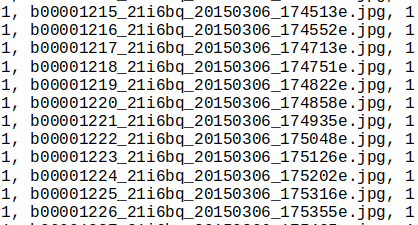
\includegraphics[scale = 0.55]{Sections/5ImageClef/images/gt_t1.png}
        \caption[Ground truth excerpt]{Excerpt of the ground truth for the dev topic 1.}  
        \label{fig:gt}
    \end{figure}

    \begin{itemize}
        \item    \textbf{Example of corresponding pictures}
    \end{itemize}
 

    The dataset is composed of nearly 200.000 images. Figure \ref{fig:gt_images} illustrates lifelog pictures from the dev topic 1 that correspond to the ground truth given in Figure \ref{fig:gt}:


    \begin{figure}[H]
        \centering
        \captionsetup{justification=centering}
        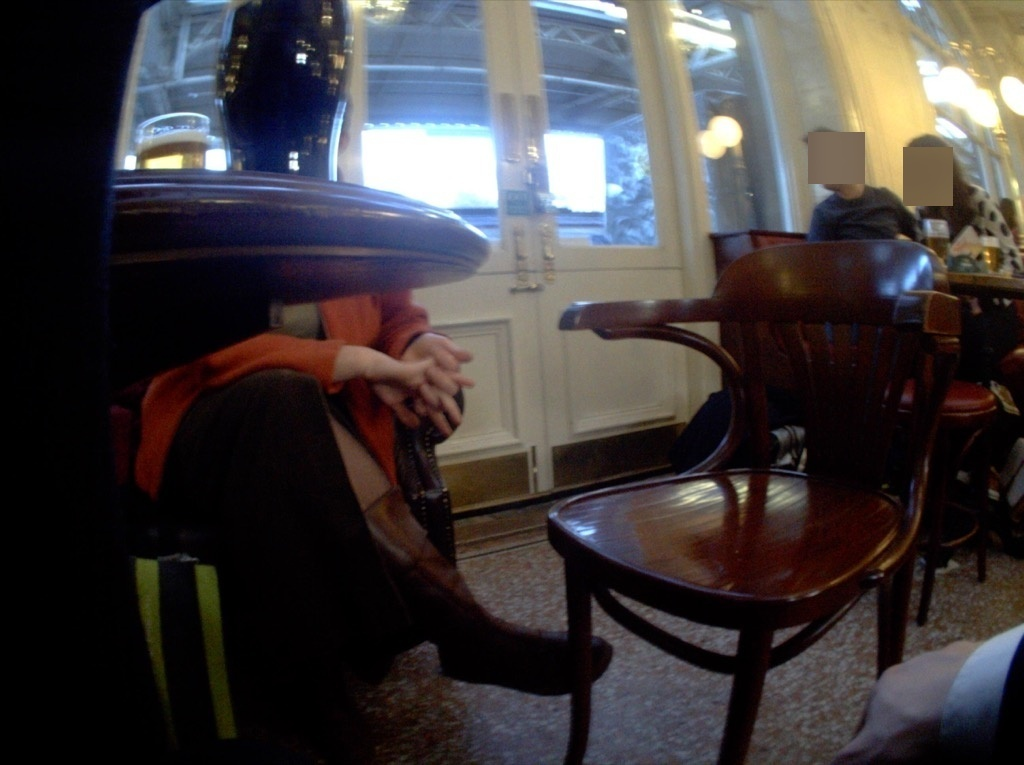
\includegraphics[width=.3\linewidth]{Sections/5ImageClef/images/example.jpg}
        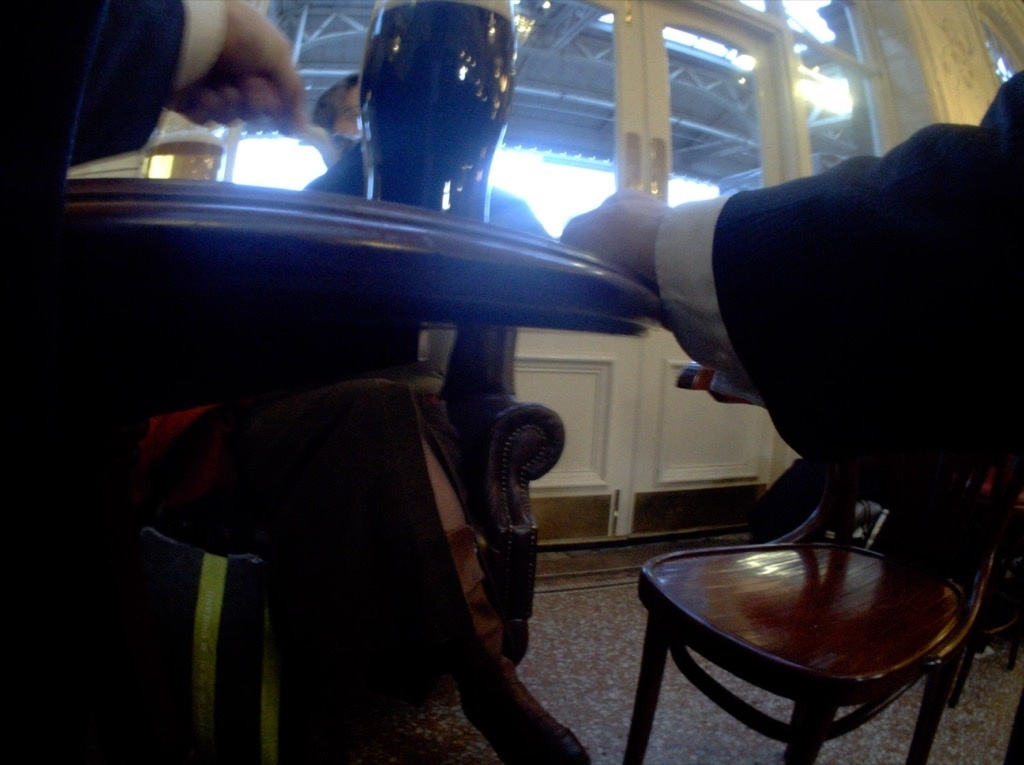
\includegraphics[width=.3\linewidth]{Sections/5ImageClef/images/example1.jpg}
        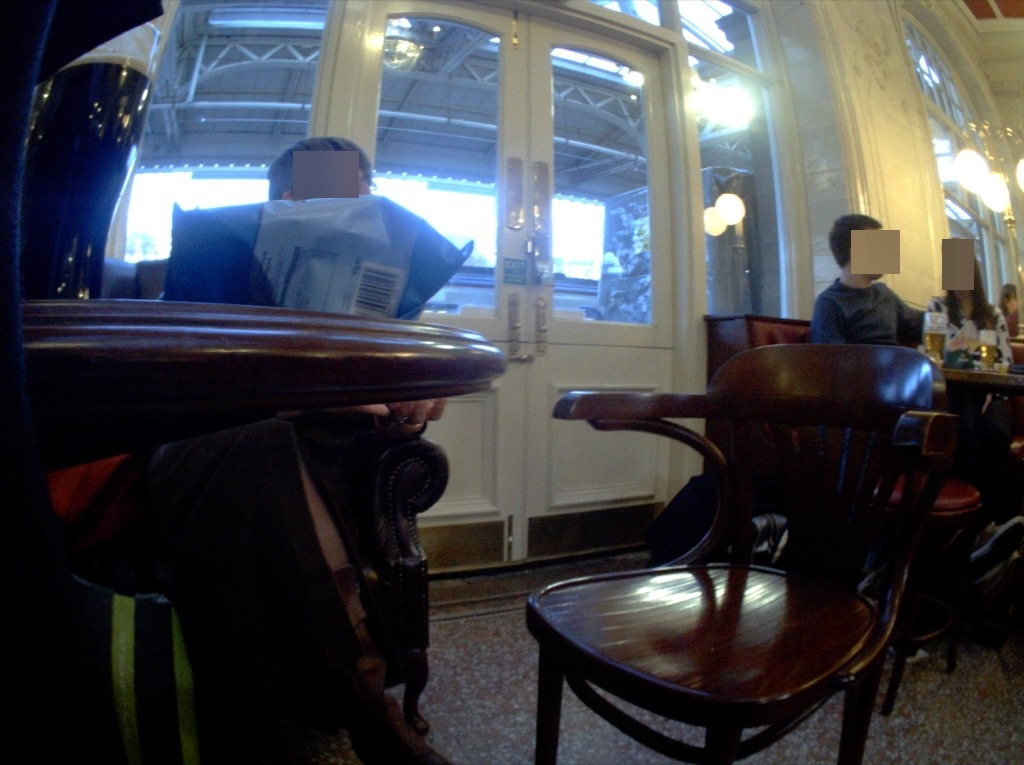
\includegraphics[width=.3\linewidth]{Sections/5ImageClef/images/example3.jpg}
        \caption[Ground truth images]{Example of 3 images that belong to the ground truth of the topic 1.}
        \label{fig:gt_images}
    \end{figure}      

    \newpage


    \subsection{Test Topic example}

    An example of one of test topics used for evaluation in the challenge the test topic 7 is presented next:

        \begin{itemize}

        \item []
        

        \textbf{Title} : \enquote{Seafood at Restaurant.}

        \textbf{Description} : \enquote{Find moments when u1 was eating seafood in a restaurant in the evening time.}

        \textbf{Narrative} : \enquote{The moments show u1 was eating seafood in any restaurant in the evening time are considered relevant. Any dish has seafood as one of its parts is also considered relevant. Some examples of the seafood can be shrimp, lobster, salmon.}

        \end{itemize}
     
    Something important to notice is that the dev and test topics share similarities in the text syntax. 

        \subsection{Evaluation Methodology}
        \label{sec:eval}
        
        
        In order to evaluate performance, the organizers use the F1-measure at X (F1@X) evaluation method. The F1-measure is the harmonic mean of both Cluster Recall at X (CR@X) metric and the Precision at X (P@X) measure. The Cluster recall is a metric that assesses how many different clusters from the ground truth are represented among the top X results  while the Precision measures the number of  relevant photos among the top X results \cite{Ninh2020}. Figure \ref{fig:ex_f1} illustrates these calculations.


        \begin{figure}[H]
            \centering
            \captionsetup{justification=centering}
            \begin{subfigure}{0.25\textwidth}
                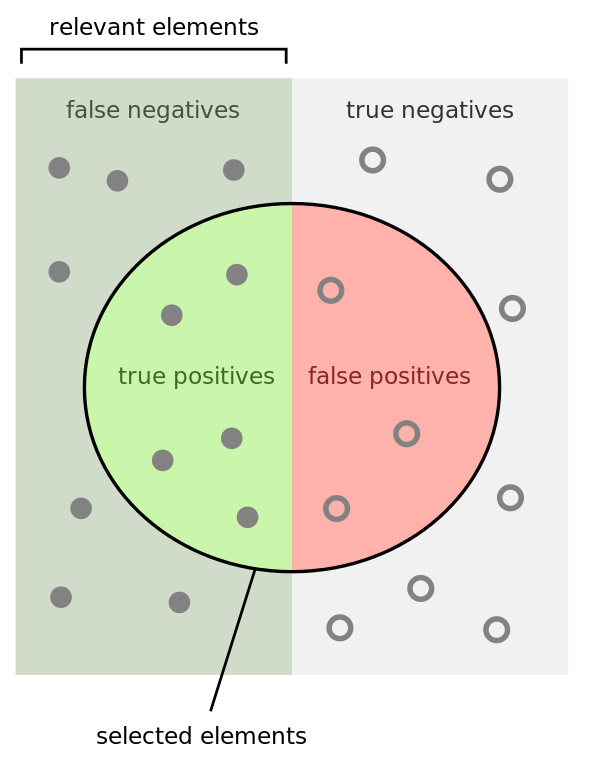
\includegraphics[width=\textwidth]{Sections/5ImageClef/images/f1_1.png}
                \end{subfigure}
                \begin{subfigure}{0.4\textwidth}
                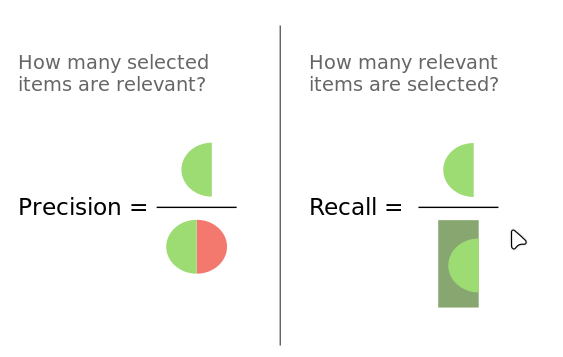
\includegraphics[width=\textwidth]{Sections/5ImageClef/images/f1_2.png}
                \end{subfigure}
            \caption[Illustration of recall and precision calculation]{Illustration of Recall and Precision calculations \cite{Wikipedia2020}.}   
            \label{fig:ex_f1}    
        \end{figure}    
           
        However, in the challenge these calculations are done as follows:

        \begin{align*}
            &\textbf{Cluster Recall at X (CR@X)}  =  N / Ngt \\ 
            &\textbf{Precision at X (P@X)} = Nr / X \\ 
            &\textbf{F1@X}  =  2\times(P@X \times CR@X)/(P@X + CR@X) \\ 
        \end{align*}

        \textit{N} is the number of image clusters represented in the first \textit{X} ranked images. \textit{Ngt} is the total number of image clusters from the ground truth. \textit{Nr} is the number of relevant pictures from the first \textit{X} ranked results.

        This year edition official rankings are obtained trough the F1-measure@10, which gives equal importance to diversity (via CR@10) and relevance (via P@10). Another important aspect of a F1-measure@10 is that only the top 10 pictures for each topic with the highest confidence score are accountable for performance assessment.



     
  
        
    \subsection{Evaluation Problems}
    \label{sec:ev_problems}

    The main problem in the evaluation of the imageCLEF lifelog subtask is that  pictures that could be considered to belong to a given moment are at times not present in the ground truth and therefore decrease the score in the F1-measure evaluation. In addition to this problem, some pictures accounted in the ground truth should have not been considered.

    Dev topic 4 is presented next to serve as an example.

    \begin{itemize}

        \item[] \textbf{Title}: \enquote{Television Recording.}

        \textbf{Description}: \enquote{Find the moments when u1 was being recorded for
        a television show.}

        \textbf{Narrative} : \enquote{To be considered relevant, there must clearly be a television camera in front of u1. The moments the interviewer/cameramen is interviewing/recording u1 are also considered relevant. This can take place at home or in another location. All recording took place in one day and in more than one location.}

    \end{itemize}


 
    \begin{figure}[H]
        \centering
        \captionsetup{justification=centering}
        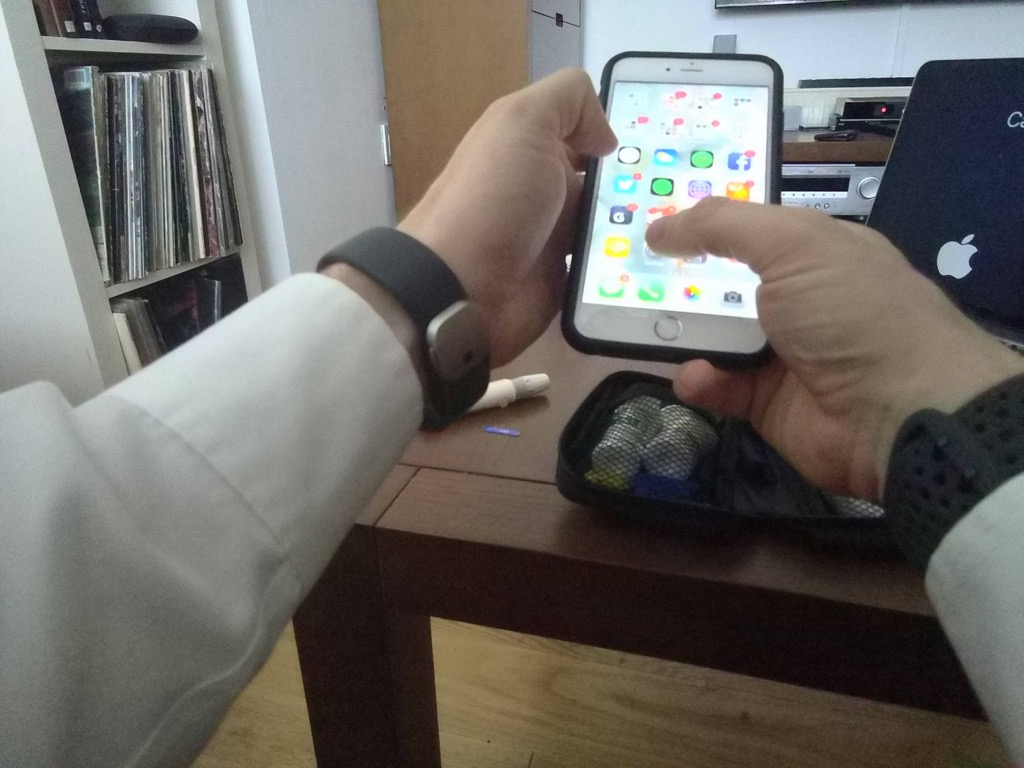
\includegraphics[width=.32\linewidth]{Sections/5ImageClef/images/2_gt.jpg}
        
\includegraphics[width=.32\linewidth]{Sections/5ImageClef/images/3_gt.jpg}
        
\includegraphics[width=.32\linewidth]{Sections/5ImageClef/images/4_gt.jpg}
        \caption[Picture that should not belong in the ground truth]{Sample of pictures that are considered in the ground truth of dev topic 4 but should not have been.}
        \label{fig:bad}
        \end{figure}


  

    \begin{figure}[H]
        \centering
        \captionsetup{justification=centering}
        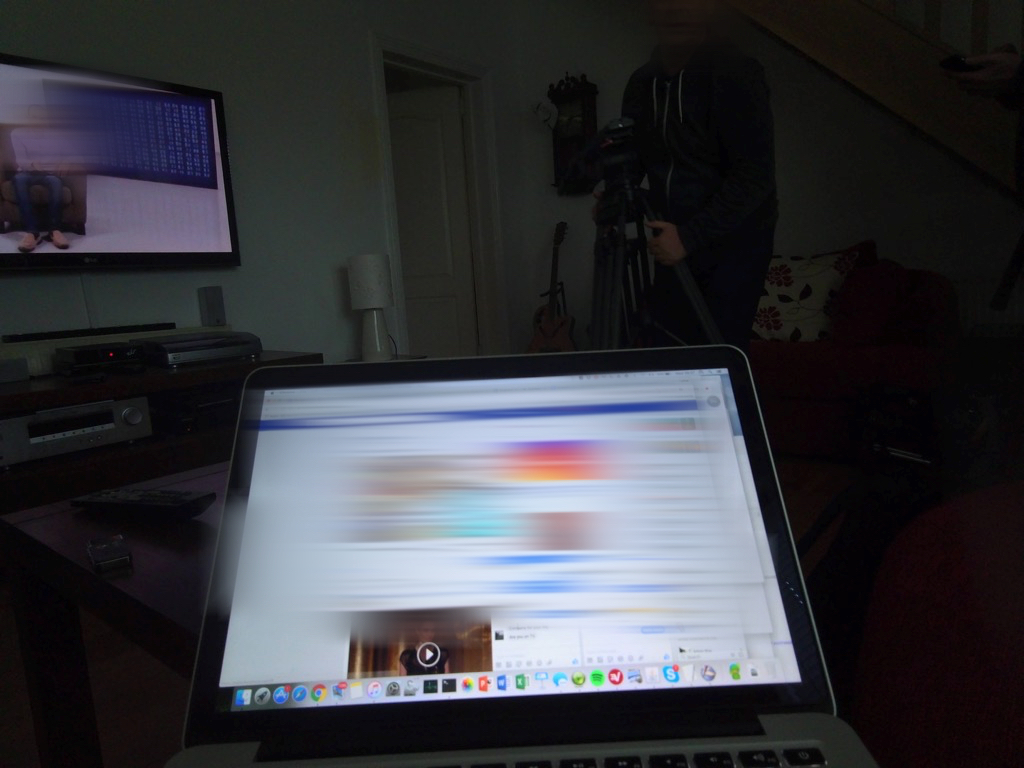
\includegraphics[width=.32\linewidth]{Sections/5ImageClef/images/1_ngt.jpg}
        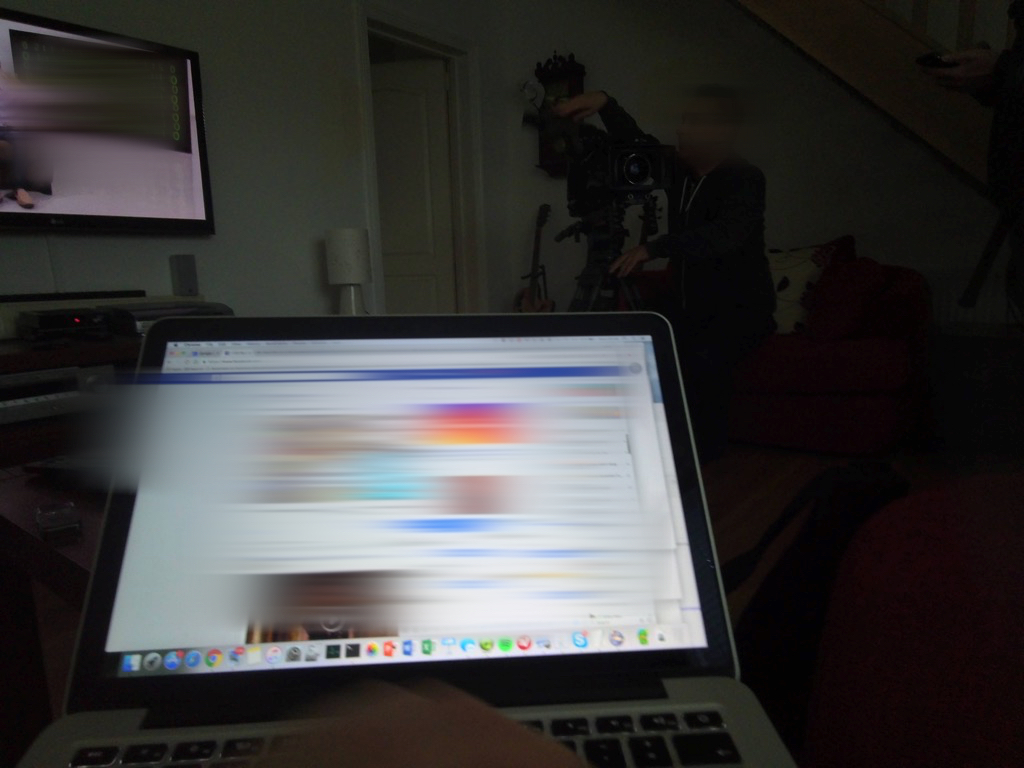
\includegraphics[width=.32\linewidth]{Sections/5ImageClef/images/2_ngt.jpg}
        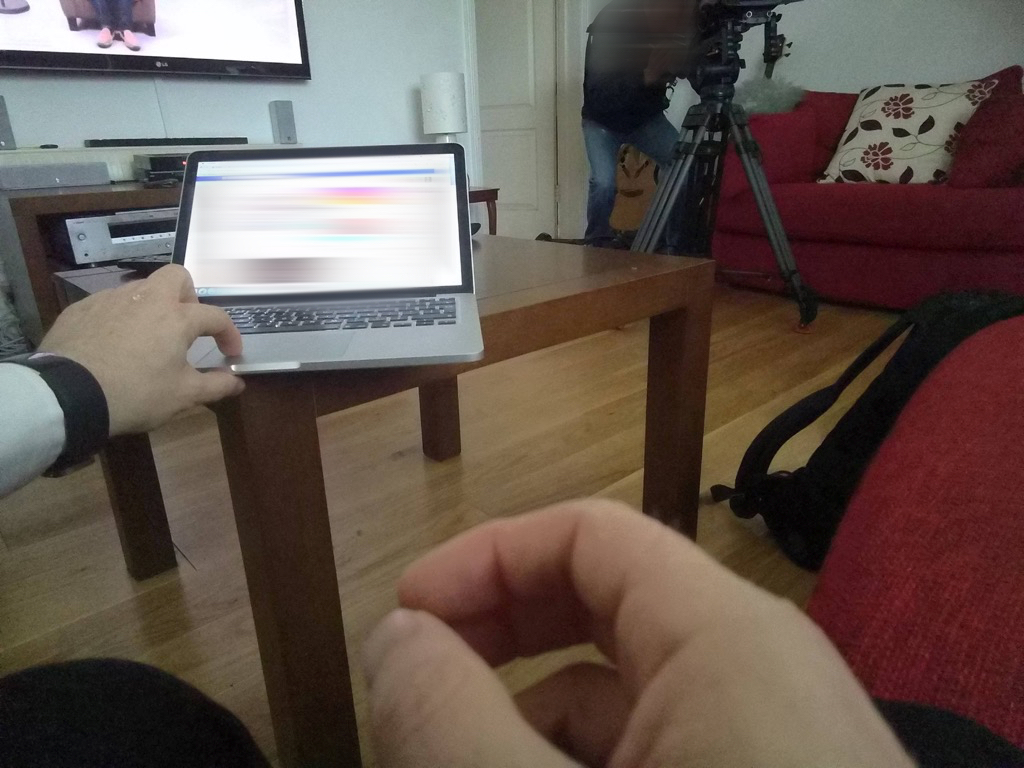
\includegraphics[width=.32\linewidth]{Sections/5ImageClef/images/3_ngt.jpg}
        \caption[Pictures that should belong in the ground truth]{Sample of pictures that were not considered in the ground truth of dev topic 4 but should have been.}
        \label{fig:good}
        \end{figure}
     
    It is clear that the pictures shown in Figure \ref{fig:bad} should not belong in the ground truth of the dev topic 4 since none of them are representative of an interview going on. The first picture shows the user on the phone, the second shows two people talking and the last picture is just a door. Finally, the images presented in Figure \ref{fig:good} should belong to the moment described in the dev topic 4 since all of them show a camera pointed at the user, however they are not.  This situation is important to have in account since the system can be retrieving images that should belong to the topic but the evaluation process just considers them wrong for not being in the ground truth. In short, this can have an impact not only in the dev topics but also in the test topics evaluation, since the ground truth is incomplete and does not present all the possible images related to a moment.
